\chapter{Computational Methods}
\label{cha:methods}

This section briefly reviews the computational methods employed in this thesis, and their advantages and limitations. Figure \ref{fig:methods} shows an overview over all employed methods, and the way they are utilized to support the mechanisms, algorithms, and cognitive models presented below. More specific and detailed descriptions of each method, including the empirical methods used to gather data for testing hypotheses for which no existing datasets could be found, are described in the respective result chapters. Chapter \ref{cha:bayespc} contains descriptions of the place cell firing data and its computational modelling, and Chapter \ref{cha:structure} the collection of data regarding spatial memory structure and accuracy data and its modelling. Chapter \ref{cha:lida} integrates the models in the same architecture, and interfaces them to a robotic simulator.

\begin{figure}[h]
	\centering
	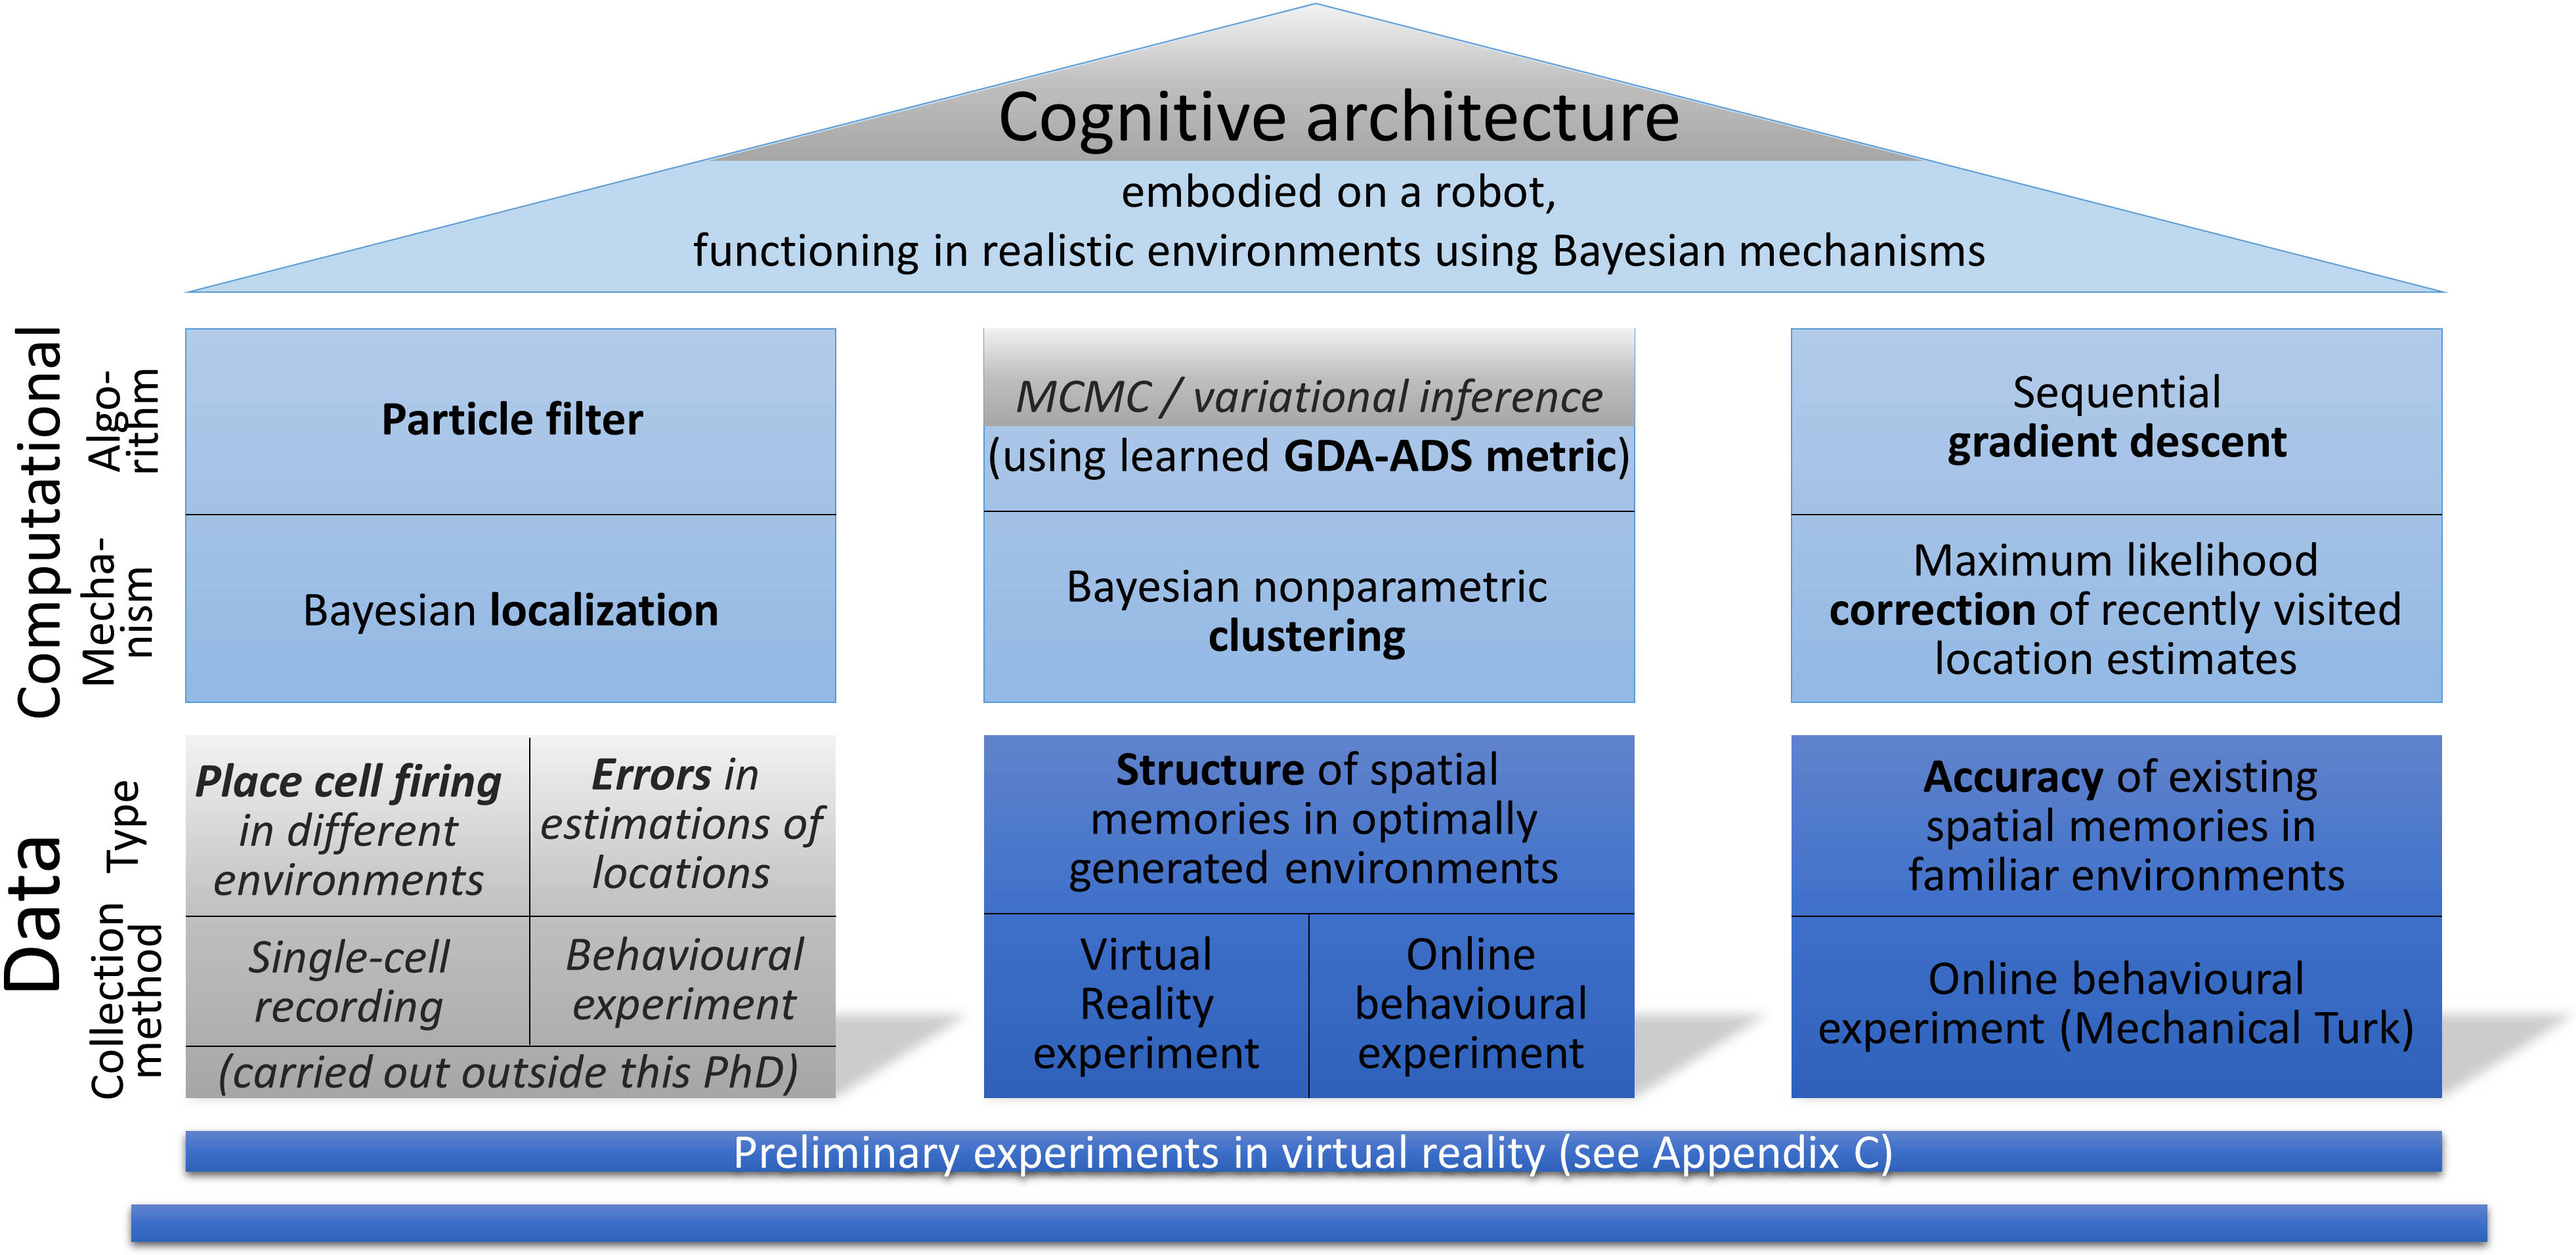
\includegraphics[width=\textwidth]{img/methodsfigure2}
	\caption[Overview of how the methods in this thesis help support real-world capable models of cognition]{\textbf{Overview of how the methods in this thesis help support real-world capable models of cognition,} roughly divided into empirical methods (bottom half) and computational methods (top half). Gray boxes with italic text contain data/code used to substantiate or implement some models, but not gathered/implemented by us.} 
	\label{fig:methods}
\end{figure}

\section{Probabilistic modelling}

Probabilistic models use probability distributions to represent quantities and the uncertainties associated with them, utilizing probability theory to manipulate these distributions \citep{ghahramani2015probabilistic}. Two basic rules provide the foundation, and together yield Bayes' theorem, which underlies Bayesian modelling. The \textit{sum rule} takes the form

\begin{equation}
\label{sumrule}
p(Y) = \sum_{X} p(Y, X),
\end{equation}

where $p(X,Y)$ is the joint probability (i.e. the probability of X and Y) and the summation is over all values which $Y$ could possibly take. $p(X)$ is also referred to as the marginal probability, and the summation in Equation \ref{sumrule} is also called marginalization (which is especially useful to make inferences about variables of interest by summing out all other variables). The \textit{product rule} states that

\begin{equation}
\label{productrule}
p(Y,X) = p(Y|X)p(X) = p(X|Y)p(Y),
\end{equation}

where $p(Y|X)$ is the conditional probability (i.e. the probability of Y given X). Combined, they yield \textit{Bayes' theorem}:

\begin{equation}
\label{bayesrule}
p(Y|X) = \frac{p(X|Y)p(Y)}{p(X)} = \frac{p(X|Y)p(Y)}{\sum_{Y} p(X, Y)}.
\end{equation}

In the context of a probabilistic model, defined by a number of parameters encoded in $Y$, and given some observed data encoded in $X$, we can use Equation \ref{bayesrule} to calculate a \textit{posterior} probability distribution of model parameters, combining \textit{prior} knowledge (or assumptions) $p(Y)$ with the \textit{likelihood} $p(X|Y)$.

The sections below summarize normative solutions to the problems required for real-world spatial cognition outlined in Chapter \ref{cha:intro} in this probabilistic framework. As mentioned there, the goal of this work is contributing to the understanding of spatial information processing in brains and minds, and not finding particularly good solutions to these problems. Numerous algorithms capable of much more accurate localization and mapping and making less restrictive assumptions have been proposed in probabilistic robotics \citep{thrun2005probabilistic}, more specifically simultaneous localization and mapping (SLAM) - see \citep{thrun2008simultaneous,durrant2006simultaneous,bailey2006simultaneous} for reviews and \citep{tuna2012evaluations} for a more recent evaluation. 

Our particular computational-level solutions for estimating locations are not novel, and very simple compared to the state of the art in SLAM. We are applying existing computational and mathematical tools to cognitive and neural mechanisms, following a long and successful history of this approach in the field of computational cognitive modelling \citep{sun2008introduction}. In this field, simplicity and restrictive approximations can be assets - a simpler, sub-optimal model which nevertheless explains empirical data better, and is more consistent with neural anatomy, is superior to an intractable or implausible optimal model at modelling cognition. Furthermore, the implementation of these abstract methods in a way consistent with the neuroscience and psychology of spatial memory is novel, as is their integration with a comprehensive cognitive architecture and their substantiation with empirical data (see Section \ref{sec:intro:outline} for the full list of novel contributions). 

\section{Bayesian cue integration}

One concrete application of Equation \ref{bayesrule} is the inference of the most likely current location of an animal, given some observations regarding the distance of a number of landmarks. For simplicity, we assume 1) a uniform prior over these observations, and 2) conditional independence of the observations given the location. The posterior probability of the current location $p(\bm x | \bm O)$, given a location prior $p(\bm x)$ and some observations $o_1, ..., o_N \in \bm O$, is 

\begin{equation}\label{bayes1}
p( \bm x | \bm O ) = \frac{p( \bm x ) p( \bm O | \bm x )}{p(\bm O)} = \gamma p( \bm x ) p( \bm O | \bm x )
\end{equation}

The prior can be obtained by adding up self-motion signals (a process called `path integration' or dead reckoning - see Chapter \ref{cha:nnreview}). Individual observation distributions can express distance measurements to landmarks, and can be multiplied due to their conditional independence:

\begin{equation}\label{bayes2}
p( \bm x | \bm O ) = \gamma p( \bm x ) \prod_{i=1}^{N} p( \bm o_i | \bm x ).
\end{equation}

For now, we further assume that each of these variables is normally distributed. This makes it straightforward to derive the variance $C_L$ of the normal/Gaussian posterior location distribution $p( \bm x | \bm O ) = \mathcal{N}(\bm x ; \mu_L, C_L)$ from the variances of the prior and of the likelihood distributions $C_x$ and $C_{o,i}$ (see e.g. \cite{wu2004properties} for the derivation of the parameters of products of Gaussian distributions):

\begin{equation}\label{bayes3}
C_{P}=(C_x^{-1}+\sum_{i=1}^{N} C_{o,i}^{-1})^{-1}
\end{equation}

In the one-dimensional case, the variance is the square of the standard deviation $\sigma$. We can say that the standard deviation of a Gaussian distribution is a measure of the `uncertainty' associated with it (as it measures the spread among possible values - the more certainly a value is known, the lower the associated $\sigma$ of the distribution describing it). Assuming that the observation uncertainties $\sigma_{o,i}$ depend linearly on the respective distances $d_{i}$, such that $\sigma_{o,i}=s \cdot d_{i}$ (Chapter \ref{cha:bayespc} provides justifications and evidence for this linear relationship), we obtain the standard deviation of the location posterior for a given set of measurement distances:

\begin{equation}\label{bayes4}
\sigma_{P}(d_1, ..., d_N)=\sqrt{(\sigma_x^{-2}+s \sum_{i=1}^{N} d_{i}^{-2})^{-1}}.
\end{equation}

Chapter \ref{cha:bayespc} uses Equation \ref{bayes4} to test the hypotheses that place cells may represent uncertainty and perform Bayesian cue integration. Although place cells constitute a two-dimensional representation, this one-dimensional treatment of observation likelihoods is an acceptable approximation in the kinds of environments from which the data was collected (rectangular boxes without landmarks, where the axes can be assumed to be independent as they are orthogonal, and a very narrow, circular track with landmarks, where the width can be neglected as it is less than $3\%$ of the length). 



%Figure \ref{fig:bayescue}

%\begin{table*}[h]
%	\centering
%	{\renewcommand{\arraystretch}{1.2}
%		\begin{tabu}{c|c}
%			$\downarrow$ {Dimensions} & {Variance of the location posterior}\\ \tabucline[3pt]{-}
%			1D & $\sigma^2_{L1D}=(\frac{1}{\sigma_x^2}+\sum_{i=1}^{N} \frac{1}{\sigma_{o,i}^2})^{-1}$ \\
%			2D & $C_{L2D}=(C_x^{-1}+\sum_{i=1}^{N} C_{o,i}^{-1})^{-1}$ \\
%		\end{tabu}
%	}
%	\caption[Variance of the posterior location estimate under Gaussian assumptions]{\textbf{Variance of the posterior location estimate under Gaussian assumptions}. $\sigma$ stands for scalar standard deviations, and $C \in \mathbb{R}^{2x2}$ for covariance matrices.}
%	\label{tbl:bayescue}
%\end{table*}

\begin{figure}[h]
	\centering
	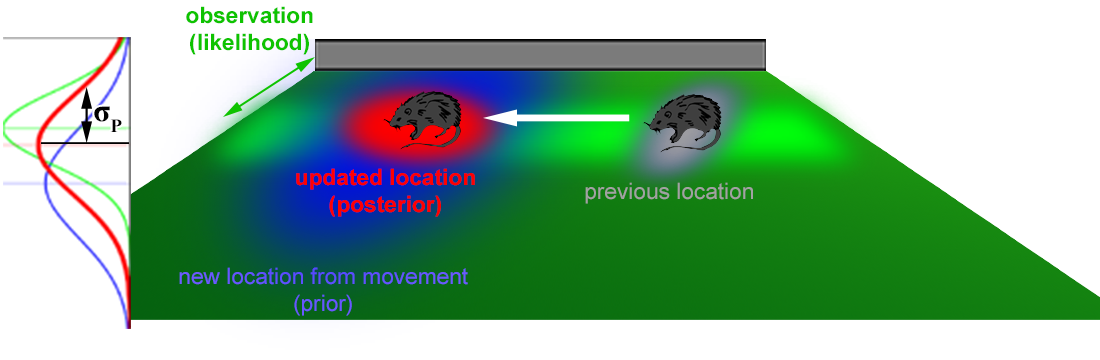
\includegraphics[width=\textwidth]{img/bayesian_localization3}
	\caption{\textbf{Bayesian cue integration for localization.} Illustration of how an animal might use its prior location belief (blue) estimated from its movement, and distance distributions e.g. to a boundary (green) to obtain a corrected location estimate (red) using Bayesian inference.} 
	\label{fig:bayescue}
\end{figure}

%
\section{Bayesian localization}

To maintain a location estimate through time, the kind of cue integration described above has to be performed regularly (after every time step). One source of location information is adding up each movement vector, a process called odometry in robotics and `path integration' in cognitive science and biology. However, movements are not accurate and noise free in real-world environments - each movement vector contains a slight error, and these errors add up over time. Eventually, these accumulating errors render the location estimate useless, if sensory information is not used to correct it. 

Bayesian localization is concerned with correcting the location estimate in time using noisy observations \citep{thrun2005probabilistic}. Conceptually, it entails performing the Bayesian cue integration to correct location estimates \textit{recursively}, after every movement / time step. Its operation can be summarized in three stages, which are performed iteratively at every time step: 1) movement (adding the current movement), 2) correction of the location estimate via Bayesian cue integration, 3) updating of the path integration estimate for use in the next iteration.

Unlike the simplified treatment above, which has considered only one snapshot in time, Bayesian localization considers the posterior at any time step $t$. This posterior distribution has to depend on all movements until now: $\bm m_{1:t}$, on all observations until now: $ O_{1:t}$, as well as the locations of known landmarks $\bm l_{1:N}$. Extended by these dependencies, the posterior location distribution from Equation \ref{bayes1} becomes

%specifying the probability distribution of the current position $ x_{t} $ given motor commands $u$, measurements $z$, and landmarks $l$. This expression can be expanded using Bayes' rule,

\begin{equation}
\label{bayesloc1}
p(\bm x_{t} | \bm m_{1:t}, \bm O_{1:t}, \bm l_{1:N}) = \gamma p(\bm O_{t} | \bm x_{t}, \bm l_{1:N}) p(\bm x_{t} | \bm m_{1:t}),
\end{equation}

through simple application of Bayes' theorem. We can use the sum rule (with the sum replaced by an integral for dealing with continuous distributions) to model the `path integration' (odometry) mechanism which provides the prior in Equation \ref{bayesloc1}:

\begin{equation}
\label{prior}
p(\bm x_{t} | \bm m_{1:t}) = \int p(\bm x_{t} | \bm x_{t-1}, \bm m_{t-1}) p(\bm x_{t-1} | \bm m_{1:t-1}) \mathrm{d} \bm x_{t-1}.
\end{equation}

This equation allows inferring the current location prior based on the most recent movement $m_{t-1}$ and on the previous location estimate $\bm x_{t-1}$ by marginalizing (integrating out) the previous location. This is a recursive formulation which yields a path integration estimate based on a starting location and a number of movements. This estimate is subject to accumulating errors. However, crucially, the corrected previous location estimate (previous posterior) can be used instead of the uncorrected previous path integration estimate. Using this insight, replacing $p(\bm x_{t-1} | \bm m_{1:t-1})$ in Equation \ref{prior} by the previous location posterior $p(\bm x_{t-1} | \bm m_{1:t-1}, \bm O_{1:t-1}, \bm l_{1:N})$ and plugging the resulting prior into Equation \ref{bayesloc1} yields

\begin{equation}
\label{bayeslocsolution}
\begin{split}
p(\bm x_{t} | \bm m_{1:t}, \bm O_{1:t}, \bm l_{1:N}) = \gamma p(\bm O_{t} | \bm x_{t}, \bm l_{1:N}) \int p(\bm x_{t} | \bm x_{t-1}, \bm m_{t-1}) \cdot \\
 p(\bm x_{t-1} | \bm m_{1:t-1}, \bm O_{1:t-1}, \bm l_{1:N}) \mathrm{d} \bm x_{t-1}
\end{split}
\end{equation}

This recursive equation for updating location estimates is a Bayes-optimal solution to the localization problem and allows inferring the current location based on two conditional densities: a model specifying the effect of movements on the location (a `motion model'):
\begin{equation}\label{motionmodelq}
p(\bm x_{t} | \bm x_{t-1}, \bm m_{t-1})
\end{equation}
and a model specifying the probability distribution of the current measurements $ \bm O_{t} $ at a position $ \bm x_{t} $ given the landmarks $ \bm l_{1:N} $ (a `sensor model'):
\begin{equation}\label{sensormodelq}
p(\bm O_{t} | \bm x_{t}, \bm l_{1:N}).
\end{equation}

Equation \ref{bayeslocsolution} is the mathematical formulation of Bayesian localization, which, conceptually, iterates over the three stages mentioned above: movement (application of the motion model), correction (via Bayes' theorem), and update.

As argued in Chapter \ref{cha:bayespc} and Appendix TODO, the activity of hippocampal place cells can be viewed as samples from probability distributions, and the size of their firing fields can be partially predicted by a Bayesian model. We will also argue based on existing evidence that the `motion model' is implemented by a neural path integrator in the entorhinal cortex, and that neurons with boundary-related firing might implement the `sensor model'.

Such a sampling-based representation of uncertainty in these spatially relevant brain areas naturally suggests employing a sequential Monte Carlo method \citep{doucet2000sequential} to computationally evaluate the integral in equation \ref{bayeslocsolution}. Although the usual method of choice in robotics is importance sampling \citep{montemerlo2007fastslam, thrun2005probabilistic}, we approximate the integral using rejection sampling \citep{doucet2000sequential}, and will argue in Chapter \ref{cha:bayespc} and Appendix TODO that coincidence detection in hippocampal place cells can implement this mechanism.

From a computational point of view, instead of inferring the parameters of the location posterior distribution (e.g. the mean and variance in case of a Gaussian), we represent it by sampling multiple location hypotheses. The mean of these hypotheses corresponds to the 'best guess' estimate, and their standard deviation to the associated uncertainty. Apart from the empirical evidence for a sampling based mechanism (see Chapter \ref{cha:bayespc}, as well as \citep{fiser2010statistically} for a more general review), the main advantage of this approach is the ability to represent free-form distributions (irregular, non-Gaussian, multimodal distributions etc.).

Particles (samples, hypotheses) $\bm x^i$ are generated regularly based on self-motion information (linear and angular movement speed $v$) according to the motion model (Equation \ref{motionmodelq}), performing path integration - in the simplest case: $ \bm x_{t}^i = \overline{\bm x}_{t-1} + \bm v'\Delta t $ - at simulated timesteps $ \Delta t $. Gaussian noise is multiplied to the estimated speed to obtain a distribution of hypotheses reflecting the path integration / odometry uncertainty (neither animals nor robots can estimate their movement speed with perfect accuracy):

$\bm v' = \bm v_{true} \cdot \mathcal{N}(1, \begin{bmatrix}\sigma_v^2 & 0\\ 0 & \sigma_\omega^2\end{bmatrix}) $,

where $ \sigma_v^2 $ and $ \sigma_\omega^2 $ are model parameters representing the variance in the linear and angular speeds, respectively. Since the estimate of $\bm v$ is noisy, accumulating errors would lead to an increase of uncertainty and the corruption of the distribution represented by the set of particles, which is why correction with the sensor model is required. 

Under Gaussian assumptions, this correction can be implemented simply by multiplying a path integration prior and a number of sensory likelihoods and solving for the means and variances (Equation \ref{bayes2}). The ensuing algorithm for Bayesian localization is trivial. When using samples instead of a Gaussian to represent the posterior, the correction can be implemented by rejection sampling \citep{doucet2000sequential}, i.e. by deleting hypotheses inconsistent with sensory measurements (see Figure \ref{fig:bayesloc}). Details regarding how brains could implement this algorithm are discussed in Chapter \ref{cha:bayespc}.

\begin{figure}[h]
	\begin{pseudocode}{movement}{samples, \textbf{v}, N}
		1: prevmean = mean(samples) \\
		2: newsamples \GETS \{ \} \\
		3: \FOREACH particle \in samples \\
		4: \quad newsamples \GETS newsamples \cup {motionModel(particle, \textbf{v})} \\
		5: \WHILE count(newsamples) < N \\
		6: \quad newsamples \GETS newsamples \cup {motionModel(prevmean, \textbf{v})} \\
		7: return(newsamples)
	\end{pseudocode}
	\begin{pseudocode}{correction}{samples, \textbf{O}, \textbf{L}}
		1: newsamples \GETS \{ \} \\
		2: \FOREACH particle \in samples \\
		3: \quad likelihood = sensorModel(particle, \textbf{O}, \textbf{L}) \\
		4: \quad \IF random() < likelihood \\
		5: \quad \quad newsamples \GETS newsamples \cup {particle} \\
		6: return(newsamples)
	\end{pseudocode}
	\begin{pseudocode}{localizationStep}{posteriorsamples, \textbf{v}, \textbf{O}, \textbf{L}, N}
		1: timestep++ \\
		2: movedsamples = movement(posteriorsamples, \textbf{v}, N) \\
		3: correctedsamples =  correction(movedsamples, \textbf{O}, \textbf{L}) \\
		4: return(correctedsamples)
	\end{pseudocode}
	\centering
	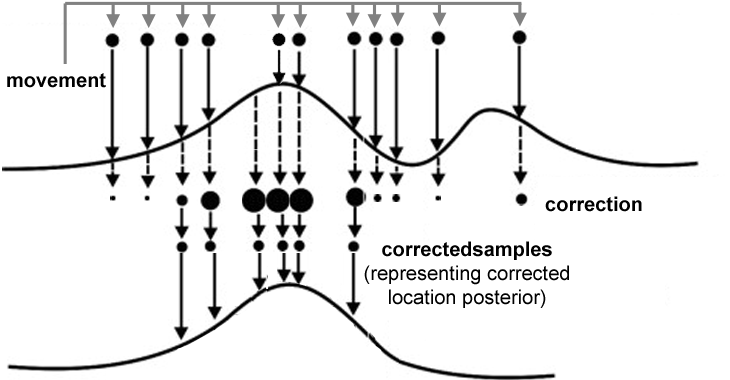
\includegraphics[width=0.75\textwidth]{img/rejectionsampling}
	\caption[Bayesian localization algorithm with rejection sampling]{\textbf{Bayesian localization algorithm with rejection sampling,} producing updated posterior samples given the samples from the previous posterior, the speed vector $\bm v$ and observations $\bm O$ at the current time step, landmarks $L$, and a particle budget $N$}
	\label{fig:bayesloc}
\end{figure}

%To correct this distribution, and to estimate the target posterior distribution \eqref{bayeslocsolution}, each particle is weighted according to the likelihood of the perceived sensory measurements from the location hypothesis represented by the particle, i.e. according to the sensor model: 
%$\bm w_t^i=p(\bm O_t|\bm x_t^i, \bm O_{t-1}, \bm m_t)$. This approach of estimating a target distribution is called importance sampling (see e.g. \cite{montemerlo2007fastslam, thrun2005probabilistic} for the derivation).

\section{Maximum likelihood map error correction}




\section{Bayesian nonparametric clustering}

%point out comp aspects WHEREVER POSSIBLE / APPROPRIATE 

%review of methods point out COMP./MATH

%point out what you can get / what you cant get, specifically saying limitations

%limitations 

%\section{Empirical methods}
%
%\subsection{Bayesian localization}
%
%The computational models presented below are based on the hypotheses summarized in Table \ref{tbl:hyp} in the Introduction. Previously gathered and published data was available for testing the hypotheses that hippocampal place cells might encode uncertainty and use it for approximate Bayesian inference, in the form of neural activity recorded using head-mounted intracranial electrodes in behaving rats in multiple environments, collected outside this PhD by \citep{burke2011influence, okeefe1996geometric, Odobescu2010} - see Chapter \ref{cha:bayespc}. Place cells also play a crucial role in human spatial memory \citep{ekstrom2003cellular}. But since the cognitive models below are concerned with human cognition, we additionally used human behaviour data published by \citep{nardini2008development} to evaluate the Bayesian localization model on a behavioural level. In this  see Chapter \ref{cha:lida}.
%
%\subsection{Bayesian nonparametric clustering}
%
%Although 
%
%\section{Computational methods}